\documentclass[a4paper, 12pt]{article}

\usepackage{exercise-sheet}
\usepackage{global-macros}
\usepackage{biblatex}
\usepackage{csquotes}
\usepackage{hyperref}
\usepackage{graphicx}
\graphicspath{{../../images}}
\usepackage{float}
\usepackage[nomarkers, figuresonly]{endfloat}

\newcommand{\by}{\boldsymbol{y}}

\hfuzz=16pt

\addbibresource{../bib/references.bib}

\title{Modelos de classificação aplicados a previsão de renda} 
\author{Professor: Rodrigo Targino \\
        Aluno: Caio Lins}
\date{\today}

\begin{document}

\maketitle

\tableofcontents

\abstract{
    Neste trabalho, utilizamos classificadores implementados na biblioteca \emph{Sci-Kit Learn}\cite{scikit-learn} para analisar alguns dados extraídos do censo populacional americano de 1994\cite{uci}, com o objetivo de prever e explicar a variável resposta, que indica se a renda anual de um indivíduo é maior ou menor que \( \$ 50 000 \).
    Após extensa validação cruzada e aplicação de técnicas para contornar a natureza desbalanceada do conjunto de dados, concluímos que a educação, a idade, as relações conjugais e os ganhos capitais externos de cada indivíduo são as variáveis que melhor explicam o \emph{target}.
    Todo o código utilizado (inclusive o que gerou este documento) pode ser encontrado \href{https://github.com/Caioflp/ML-final-project.git}{neste repositório}.
}

\section{\emph{Recap} do conjunto de dados}

Relembrando o que foi apresentado no relatório anterior, estamos trabalhando com o \emph{``Census Income Data Set''}~\cite{uci}.
Nossa tarefa é classificar cada indivíduo que participou do censo com relação à sua renda: se ele ganha mais que \$ 50 000 por ano, ou não.
À nossa disposição, temos uma série de variáveis de caráter socioeconômico, categóricas e quantitativas, dentre as quais gostaríamos de identificar aquelas que melhor explicam a variável resposta.
Para tanto, treinamos, no nosso conjunto de dados, modelos de classificação que possuem uma boa explicabilidade, ou seja, que não são modelos do tipo ``caixa preta''.
Foram eles, em ordem crescente de complexidade: \emph{perceptron}, regressão logística, modelos baseados em árvores (uma árvore, \emph{bagging} e \emph{random forest}) e \emph{support vector machines (SVM)}.

\subsection{\emph{Old problems and new}}

No último relatório foi apontado que o conjunto de dados apresentava algumas lacunas, em três \emph{features} diferentes.
Apesar de, inicialmente, termos considerado utilizar técnicas estatísticas para preencher os dados, como, por exemplo, o algoritmo EM, por uma questão de (falta de) recursos humanos não foi possível implementar essa ideia.
A solução utilizada foi a mais simples: descartamos as amostras que possuíam alguma \emph{feature} faltante.
Como elas eram poucas (\( \sim 2800 \), contra as \( \sim 48 000 \) totais), isso não representou uma perda muito significativa.

Entretanto, uma questão não considerada anteriormente se apresentou quando começamos as treinar modelos: o \textbf{desbalanceamento do \emph{dataset}}.
A proporção entre instâncias positivas (ganham mais que 50K) e negativas é de, aproximadamente, 1:3, ou seja, \( \sim 25 \% \) dos indivíduos tem renda elevada.
Apesar de não ser exageradamente expressiva, essa assimetria faz com que haja uma tendência para classificar uma determinada instância como negativa.

Ressaltamos que isso não necessariamente é um problema, pois tudo depende de qual é o objetivo da análise que está sendo conduzida.
Se a proporção entre classes fora do \emph{dataset} é a mesma de dentro \emph{dataset} e, por algum motivo, deseja-se apenas obter o modelo com melhor \emph{score}
\footnote{Proporção de instâncias classificadas corretamente.},
não importa muito se há um forte viés para alguma das classes.
Entretanto, raramente esse é o caso em aplicações reais de \emph{machine learning}.
No nosso problema, por exemplo, não é útil que todos os coeficientes da regressão logística sejam muito baixos, pois isso diz pouco sobre a relevância de cada um para explicar a variável resposta.
Portanto, foi necessário utilizar uma estratégia para contrabalancear o viés no conjunto de dados.

\section{Metodologia utilizada}

O problema de ter um \emph{dataset} desbalanceado é muito comum, e portanto, existem algumas formas já consolidadas de contorná-lo.
Duas dessas técnicas são o \emph{over sampling} e \emph{under sampling}.
Na primeira, acrescenta-se, artificialemente, mais instâncias da classe menos respresentada ao \emph{dataset}.
Isso pode ser feito repetindo instâncias já conhecidas, ou criando instâncias sintéticas.
Na segunda, remove-se instâncias pertencentes a classes dominantes.
Apesar de bastante comumns para resolver esse tipo de problema, essas duas alternativas não foram utilizadas.

A estratégia que utilizamos para contrapor o viés do conjunto de dados envolveu duas components.
Primeiramente, selecionamos os hiperparâmetros de cada modelo com um \emph{grid search cross validation}, tomando como referência uma métrica diferente do \emph{score}, que levasse em conta o desempenho dele nas duas classes.
As métricas escolhidas foram a \textbf{AUC} (\emph{Area Under Curve}), que mede a área debaixo da curva \textbf{ROC} (\emph{Receiver Operating Characteristic}), e, no caso do SVM (que não estima probabilidades), a \emph{balanced accuracy score}, que corresponde à média aritmética entre o \emph{recall}
\footnote{\emph{Score} dentro de uma dada classe. Em classificação binária, se refere ao \emph{score} para a classe positiva.}
e a especificidade
\footnote{\emph{Recall} para a classe negativa.}.
Utilizamos a média aritmética por não termos motivações reais para priorizar o \emph{recall} ou a especificidade.

Em segundo lugar, durante o treino de cada modelo, utilizamos pesos diferentes para as duas classes.
Essa abordagem já está implementada nos estimadores do \emph{Sci-Kit Learn} (ao especificar o hiperparâmetro \verb|class_weights = "balanced"|) e corresponde a multiplicar as perdas individuais por um peso específico da classe verdadeira da instância.
Para exemplificar essa abordagem e como o cálculo dos pesos é feito, utilizamos~\cite[Páginas 144-5]{king01} como referência, o mesmo artigo utilizado como base pelos desenvolvedores do \emph{Sci Kit Learn} para implementar essa funcionalidade, como pode-se ver \href{https://scikit-learn.org/stable/modules/generated/sklearn.utils.class_weight.compute_class_weight.html}{aqui}.

Suponha que estamos realizando uma regressão logística.
Denotamos por \( \pi_{ i } \) a probabilidade estimada pelo modelo de que a \( i \)-ésima instância de treino seja positiva, por \( \beta \) os pesos do modelo e por \( y_{ i } \) a variável resposta.
Então a log-verossimilhança dos dados é dada por
\begin{equation*}
    \log L ( \beta \mid \by ) = \sum_{ y_{ i } = 1 } \log \pi_{ i }
    + \sum_{ y_{ i } - 0 } \log ( 1 - \pi_{ i } )
.\end{equation*}
Supondo que a proporção real de ocorrência do evento estudado é \( \tau \in [0, 1] \) e a proporção no conjunto de dados é \( \overline{ y } \), a log-verossimilhança ponderada pelos pesos \( w = \left\{ w_{ 0 }, w_{ 1 } \right\} \) é dada por
\begin{equation*}
    \log_{ w } L ( \beta \mid \by ) =
    w_{ 1 } \sum_{ y_{ i } = 1 } \log \pi_{ i } + w_{ 0 } \sum_{ y_{ i } = 0 } \log ( 1 - \pi_{ i } )
,\end{equation*}
onde \( w_{ 1 } = \tau / \overline{ y } \) e \( w_{ 0 } = ( 1 - \tau ) / ( 1 - \overline{ y } ) \).
Ao dividir pela proporção no \emph{dataset} e multiplicar pela proporção real, estamos corrigindo o viés provocado pela amostragem.
A extensão para múltiplas classes é feita de maneira análoga.
Outro link que pode ser de ajuda para entender a ideia do balanceamento é \href{https://github.com/scikit-learn/scikit-learn/issues/4324}{este}.

Na implementação do \emph{Sci-Kit Learn}, como é possível ver no link já apresentado, pressupõe-se que, fora do \emph{dataset}, todas as classes possuem a mesma frequência, o que podemos pressupor, com segurança, não ser verdade no nosso caso.
Entretanto, ao realizar validação cruzada, vemos que, para \textbf{quase todos os modelos testados}, a versão com pesos se saiu melhor do que a versão sem pesos.

\subsection{Abordagem geral}

Feita essa discussão sobre dados desbalanceados, especificiamos agora qual foi a abordagem geral para treinar os modelos.
Inicialmente, separamos \( 25\% \) dos dados para teste e o restante para treino.
O dado de teste só foi utilizado para computar os resultados apresentados na seção seguinte.
Em seguida, como mencionamos anteriormente, selecionamos os melhores hiperparâmetros para cada modelo com um \emph{grid search cross validation}, por meio de uma função disponível no \emph{Sci-Kit Learn}.
Procuramos explorar ao máximo o espaço de hiperparâmetros, dados os recursos computacionais disponíveis.

\section{Resultados dos Modelos}

\subsection{Perceptron}

O perceptron é o modelo linear mais simples, pois apenas realiza uma combinação linear das \emph{features} e classifica o indivíduo de acordo com o sinal do resultado.
O melhor modelo encontrado utiliza regularização do tipo \emph{elastic-net}, com peso para regularização de Lasso igual a \( 0.3 \).
O peso para a regularização como um todo foi \( 0.001 \).

Na Figura \ref{perceptron metric} podemos ver a matriz de confusão e a curva ROC para este modelo.
As principais métricas do modelo foram:
\begin{itemize}
    \item \emph{Recall}: \( 90.7 \% \).
    \item Precisão: \( 32.8 \% \).
    \item Especificidade: \( 38.8 \% \).
    \item AUC: \( 0.648 \) (0.852 no treino).
\end{itemize}
\begin{figure}[htb]
    \begin{center}
        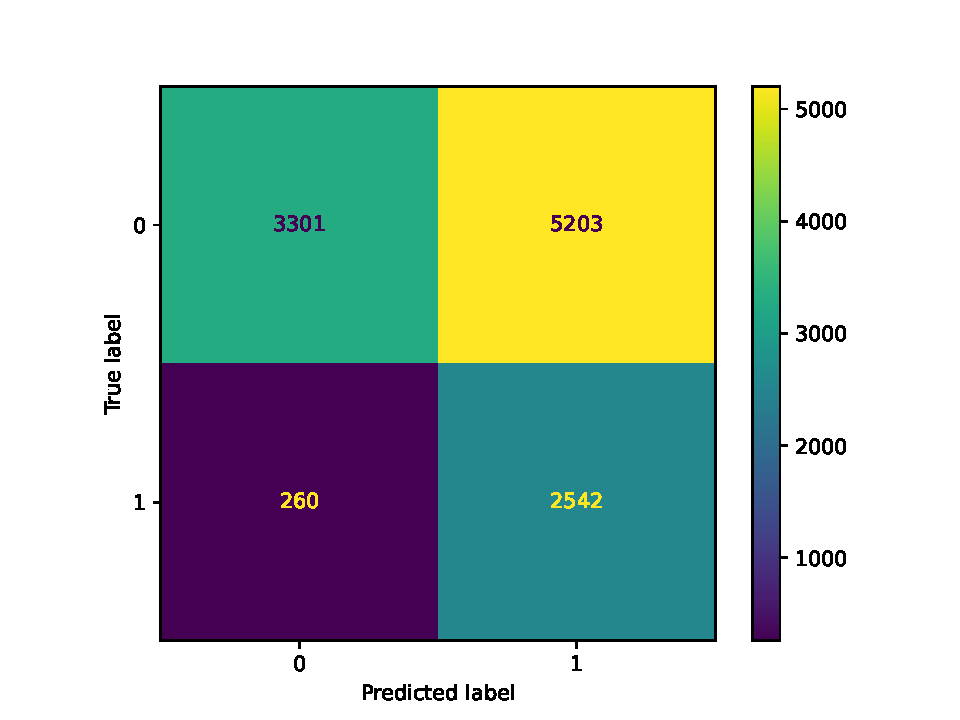
\includegraphics[width=.6\textwidth]{matrix_perceptron.pdf} \\
        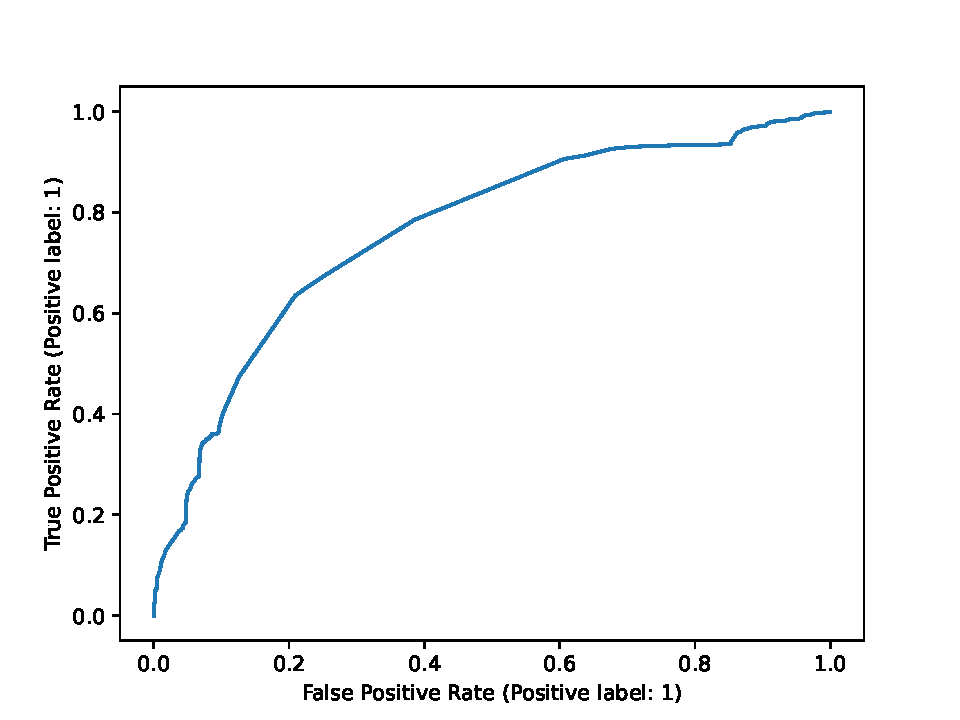
\includegraphics[width=.6\textwidth]{roc_curve_perceptron.pdf}
    \end{center}
    \caption{Matriz de confusão e curva ROC para o modelo perceptron. AUC = 0.648.}
    \label{perceptron metric}
\end{figure}

Para que os coeficientes tivessem valores significativos, o perceptron foi treinado com dados devidamente padronizados, para terem média zero e variância \( 1 \).
As \emph{features} com maiores pesos estão representadas na Figura \ref{perceptron feature}.
\begin{figure}[htb]
    \begin{center}
        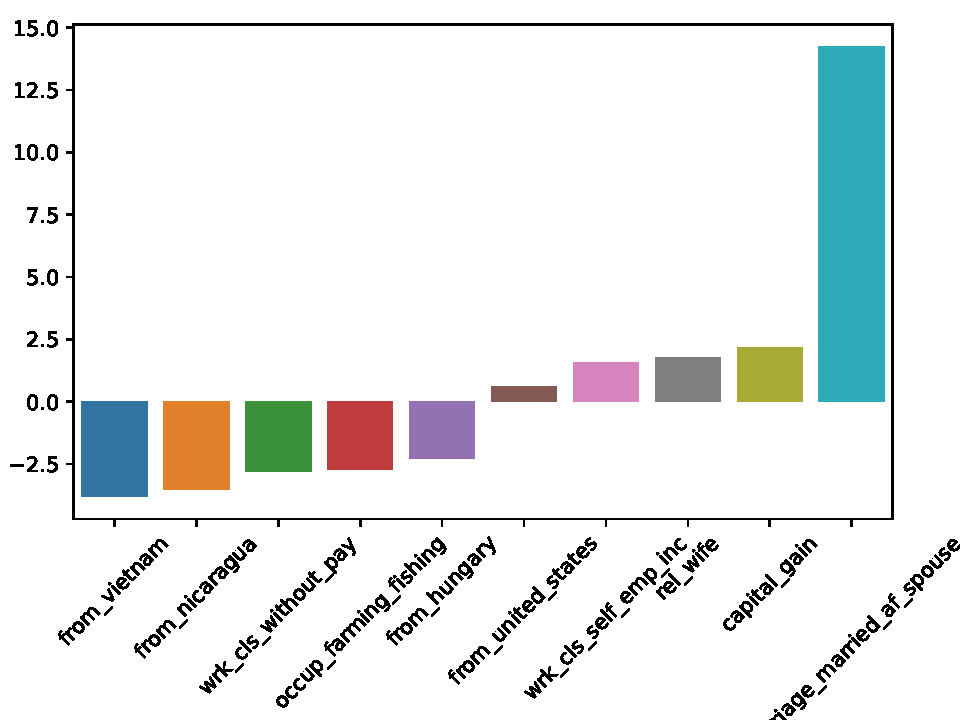
\includegraphics[width=.7\textwidth]{coefs_perceptron.pdf}
    \end{center}
    \caption{Feautures com maiores valores absolutos de pesos, positivos e negativos, para o perceptron.}
    \label{perceptron feature}
\end{figure}
Podemos ver claramente que, de acordo com o perceptron, ter um cônjuge nas forças aramadas (\verb|af| significa \emph{armed forces}) contribui de forma positiva para ter uma renda alta, enquanto ser do Vietnã, de forma negativa.
O campo \verb|capital_gain| não estava muito bem explicado na fonte do dataset, porém é razoável assumir que se trata dos ganhos monetários de fontes além do salário, como investimentos, por exemplo.

\subsection{Regressão Logística}

A Regressão Logística já é um modelo um pouco mais sofisticado, por usar uma ativação não linear.
Também utilizamos um \emph{Scaler} para padronizar os dados antes de cada chamada ao método \emph{fit}, de modo que os coeficientes possam ser utilizados para medir a relevância das \emph{features}.
O melhor modelo encontrado utiliza regularização do tipo \emph{elastic-net}, com peso para regularização de Lasso igual a \( 0.25 \).
A forma como o peso é dado para a regularazição como um todo é diferente do perceptron.
O termo da perda correspondente aos dados é multiplicado por uma constante \( C \), que, no caso do modelo validado, foi igual a \( 0.01 \), o que significa uma regularização bastante elevada.

Na Figura \ref{logit metric} podemos ver a matriz de confusão e a curva ROC para este modelo.
As principais métricas do modelo foram:
\begin{itemize}
    \item \emph{Recall}: \( 91.5 \% \).
    \item Precisão: \( 50.8 \% \).
    \item Especificidade: \( 70.7 \% \).
    \item AUC: \( 0.901 \) (0.904 no treino).
\end{itemize}
\begin{figure}[htb]
    \begin{center}
        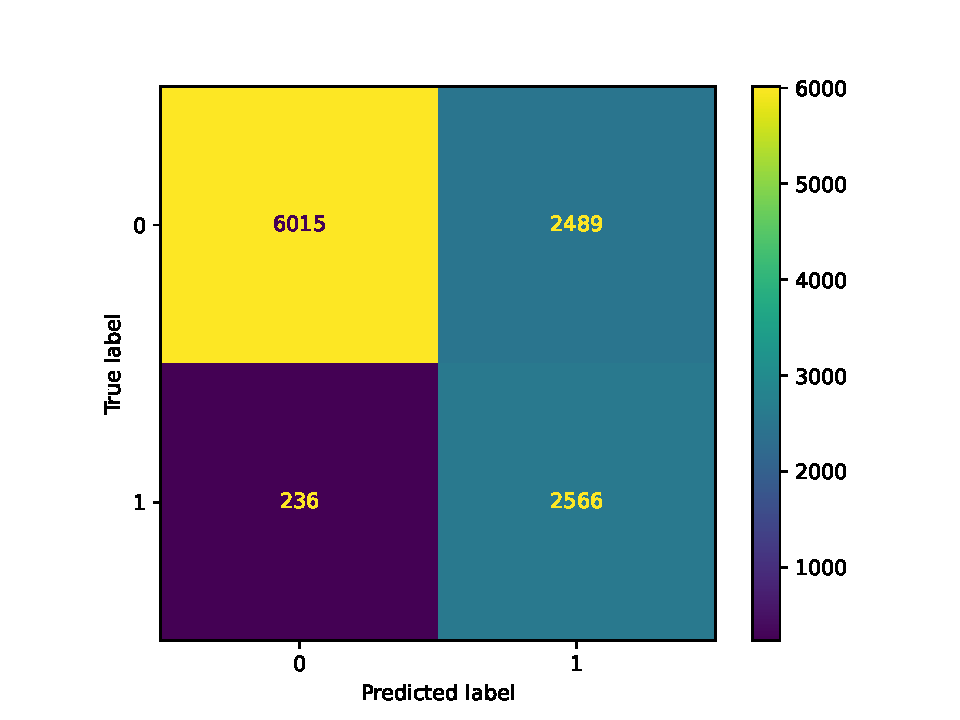
\includegraphics[width=.6\textwidth]{matrix_logit.pdf} \\
        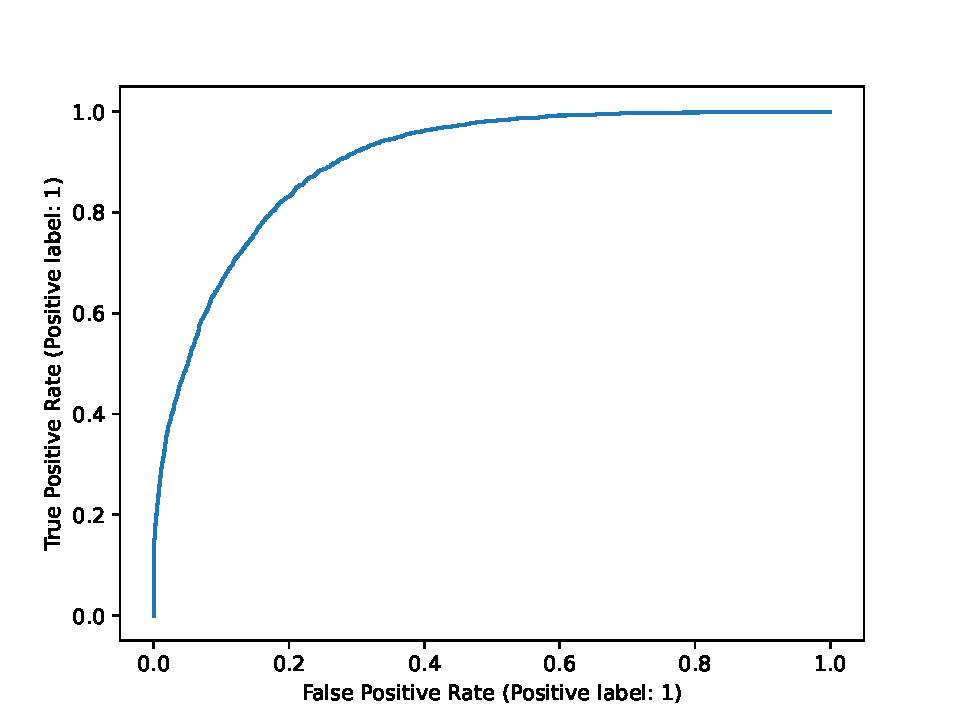
\includegraphics[width=.6\textwidth]{roc_curve_logit.pdf}
    \end{center}
    \caption{Matriz de confusão e curva ROC para o modelo de regressão logística. AUC = 0.901.}
    \label{logit metric}
\end{figure}
As \emph{features} com maiores pesos estão representadas na Figura \ref{logit feature}.
Por ela, concluímos que ter elevados ganhos de renda além do salário (\verb|capital_gain|), bem como ter uma boa educação, são fatores que contribuem para uma ter uma elevada renda.
Por outro lado, nunca ter se casado (\verb|marriage_never_married|) contribui negativamente.
\begin{figure}[htb]
    \begin{center}
        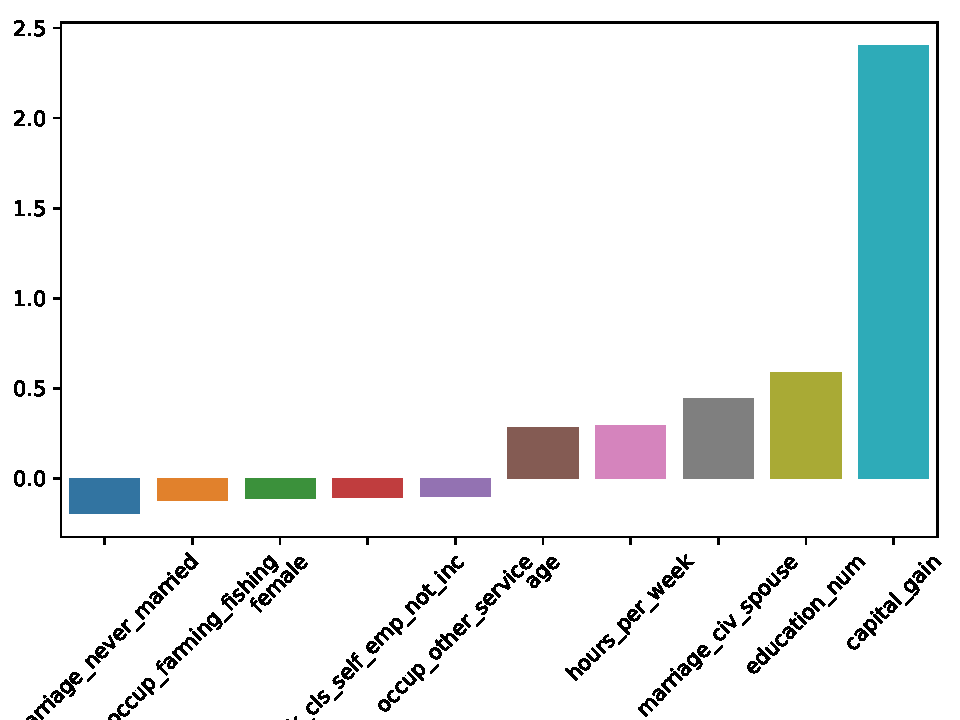
\includegraphics[width=.7\textwidth]{coefs_logit.pdf}
    \end{center}
    \caption{Feautures com maiores valores absolutos de pesos pesos, positivos e negativos, para a regressão logística.}
    \label{logit feature}
\end{figure}

\subsection{Modelos baseados em árvores}

Para os modelos baseados em árvores, uma desvantagem comparativa foi o fato de que a implementação de árvores do \emph{Sci-Kit Learn} não suporta \emph{features} binárias, como é possível ver no último parágrafo \href{https://scikit-learn.org/stable/modules/tree.html#tree-algorithms-id3-c4-5-c5-0-and-cart}{desta seção (1.10.6)} do \emph{user guide} do \emph{Sci-Kit Learn}.
Para confirmar isso, ao tentarmos treinar com variáveis categóricas, geramos uma falha, pois o algoritmo esparava apenas floats.

\subsubsection{Uma árvore}

Com o intuito de começar simples e depois complicar, primeiro treinamos uma única árvore.
Os melhores parâmetros escolhidos por validação cruzada foram:
\begin{itemize}
    \item Um \( \alpha \) relativo à poda de custo-complexidade igual a \( 0.001 \).
    \item  Profundidade máxima igual a \( 9 \).
    \item Um mínimo de \( 1 \% \) de samples em cada folha.
\end{itemize}

Na Figura \ref{single tree metric} podemos ver a matriz de confusão e a curva ROC para este modelo.
As principais métricas do modelo foram:
\begin{itemize}
    \item \emph{Recall}: \( 49.9 \% \).
    \item Precisão: \( 70.2 \% \).
    \item Especificidade: \( 93.0 \% \).
    \item AUC: \( 0.84 \) (0.844 no treino).
\end{itemize}
\begin{figure}[htb]
    \begin{center}
        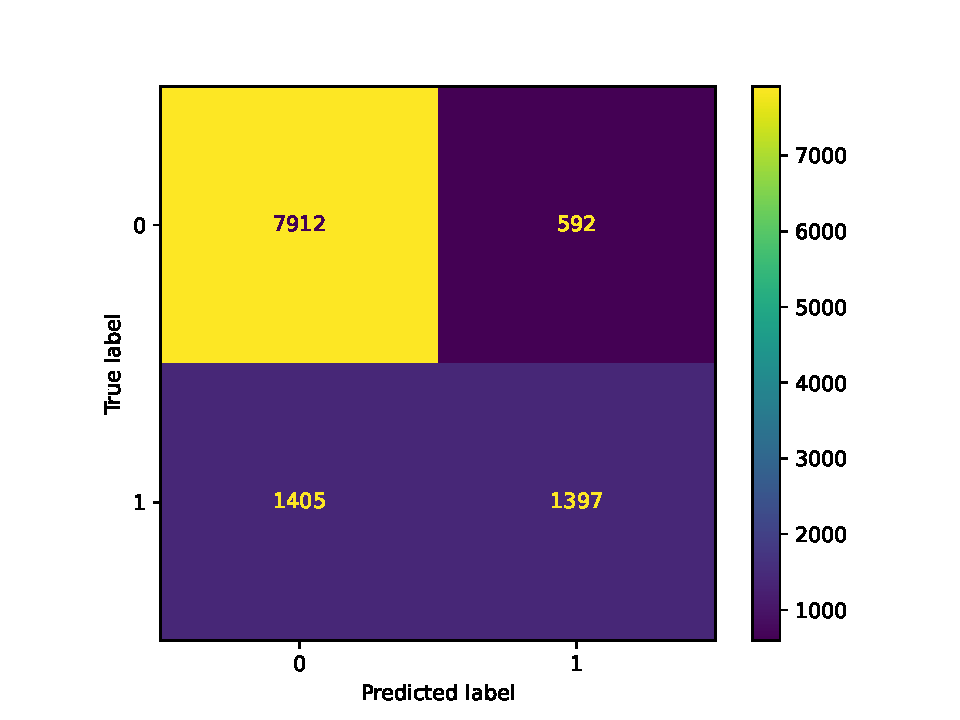
\includegraphics[width=.6\textwidth]{matrix_single_tree.pdf} \\
        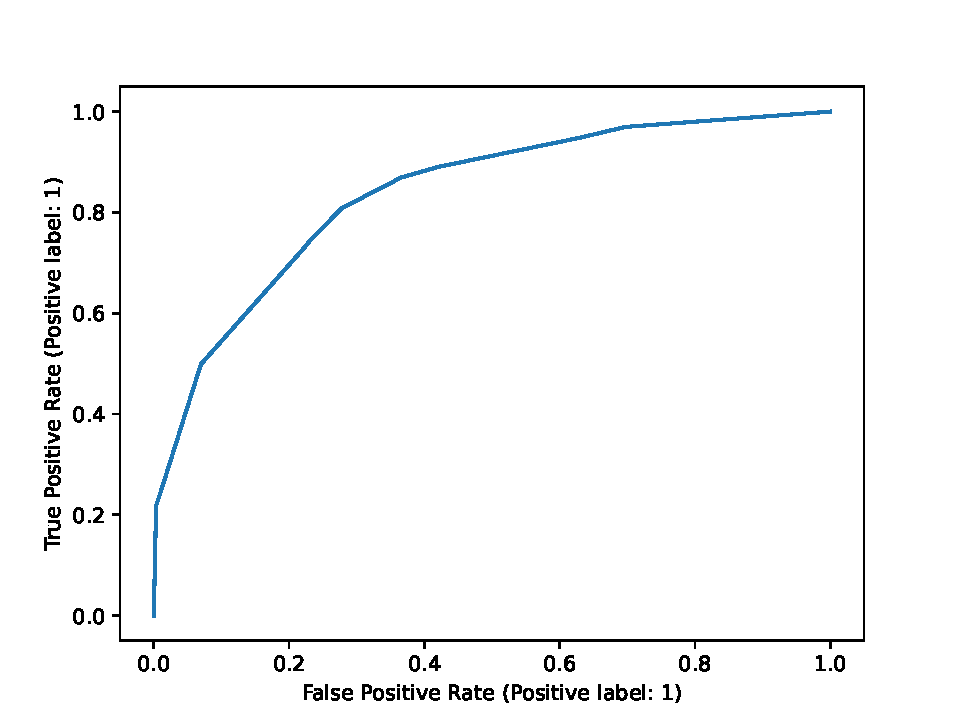
\includegraphics[width=.6\textwidth]{roc_curve_single_tree.pdf}
    \end{center}
    \caption{Matriz de confusão e curva ROC para uma única árvore. AUC = 0.838.}
    \label{single tree metric}
\end{figure}

As \emph{features} com mais importância estão retratadas na Figura \ref{single tree feature}.
Essa importância é calculada como sendo a redução total da perda, normalizada, causada por aquela \emph{feature}.
Podemos ver que, de acordo com uma única árvore, o grau de educação de um indivíduo e a sua idade são duas boas variáveis para explicar a sua renda.
\begin{figure}[htb]
    \begin{center}
        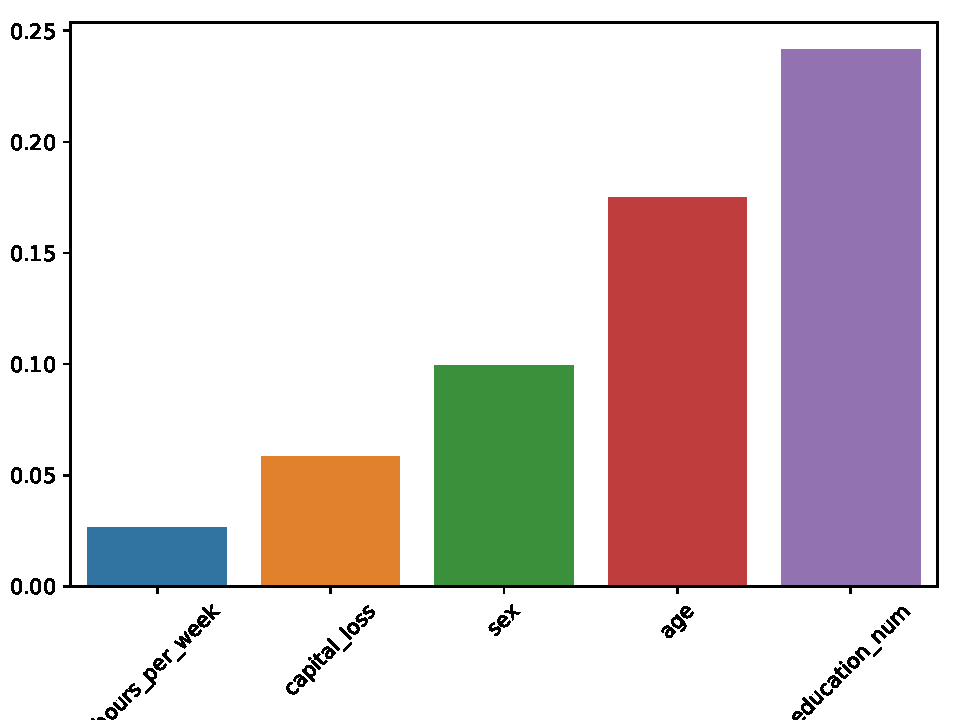
\includegraphics[width=.7\textwidth]{single_tree_feature_importances.pdf}
    \end{center}
    \caption{Features com maiores importâncias, de acordo com uma única árvore.}
    \label{single tree feature}
\end{figure}
Por se tratar de apenas \emph{uma} árvore, podemos representá-la graficamente, o que é feito na Figura \ref{plot tree}
\begin{figure}[htb]
    \begin{center}
        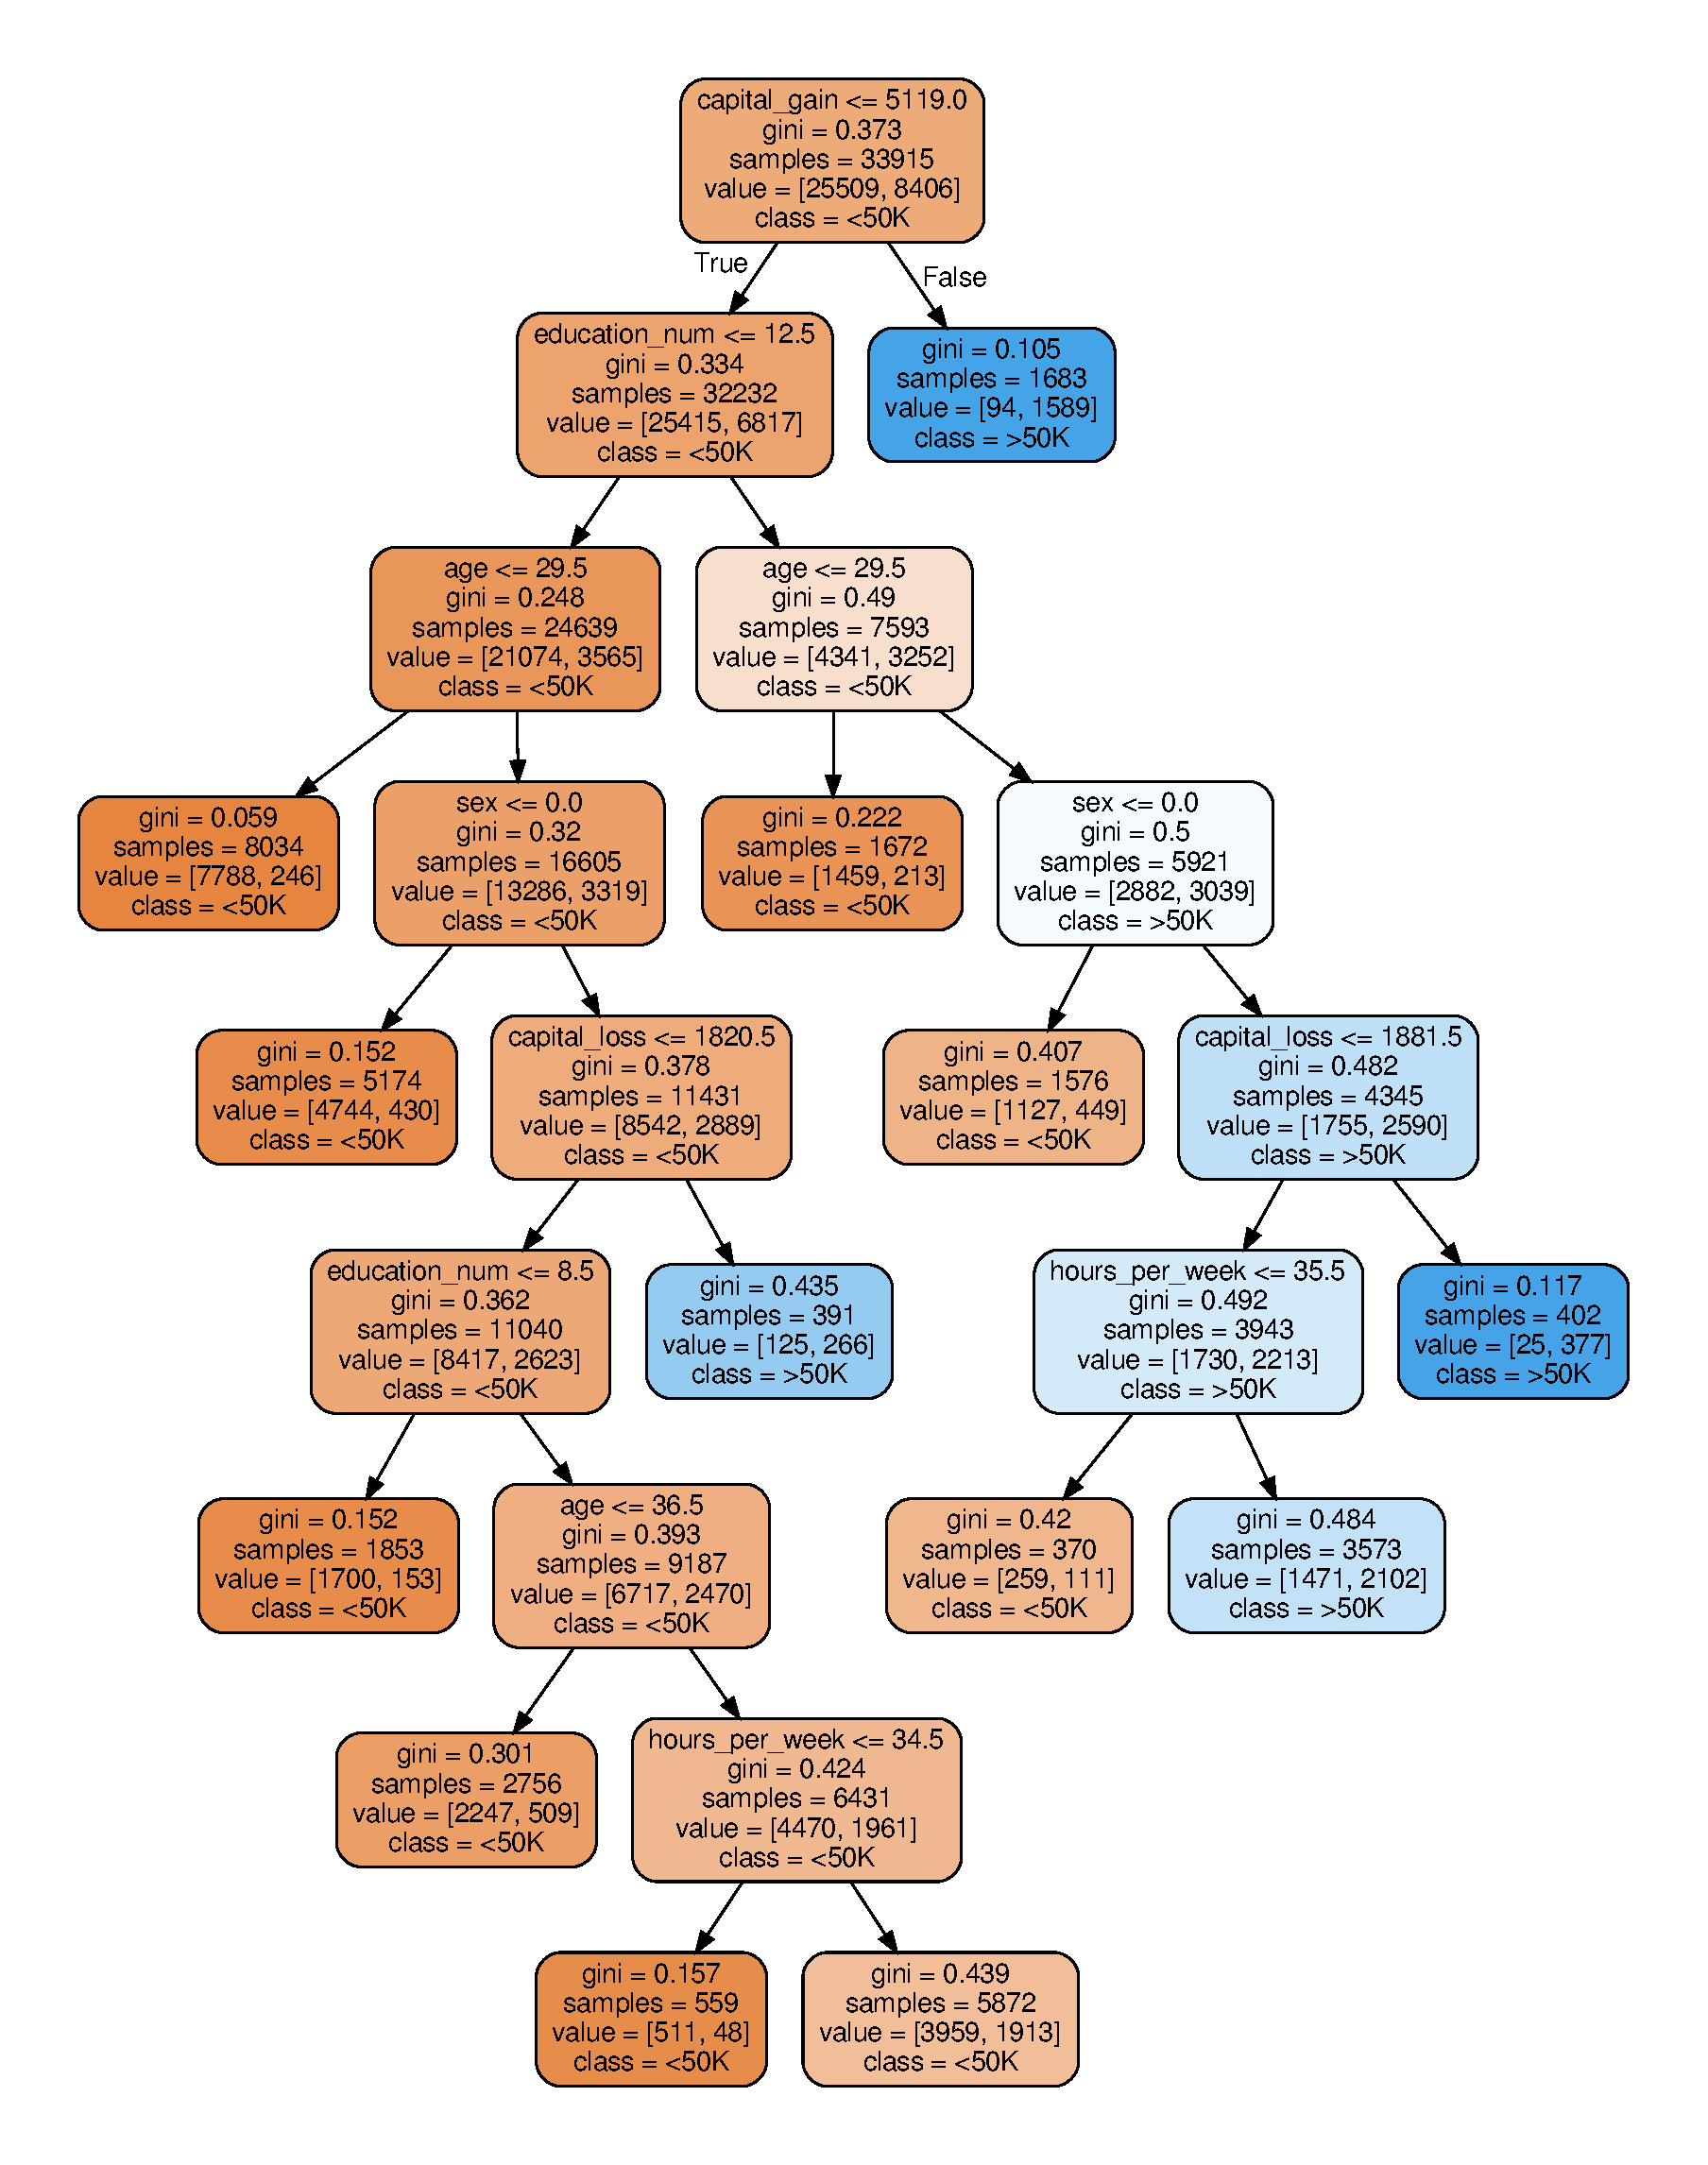
\includegraphics[width=\textwidth]{tree/Source.gv.pdf}
    \end{center}
    \caption{Árvore obtidas ao fitarmos apenas um classificador no dataset.}
    \label{plot tree}
\end{figure}

\subsubsection{\emph{Bag of trees}}

O próximo passo é o de ajustar um \emph{bagging} classifier nos dados, utilizando árvores como classificadores básicos.
Esse tipo de estimdor tem como objetivo reduzir a variância do modelo, de modo que se espera que ele generalize melhor.
Por uma questão de falta de recursos computacionais, como parâmetros para cada classificador dentro do \emph{bag}, utilizamos os melhores parâmetros encontrados por validação cruzada para uma única árvore.
Com relação ao número de estimadores, vemos que, como esperado, quanto mais estimadores utilizamos, melhor é o desempenho do modelo.
Entretanto, a partir de cerca de \( 100 \) estimadores, o ganho marginal começou a ser muito pequeno.

Na Figura \ref{bag of trees metric} podemos ver a matriz de confusão e a curva ROC para este modelo.
As principais métricas do modelo foram:
\begin{itemize}
    \item \emph{Recall}: \( 27.4 \% \).
    \item Precisão: \( 89.1 \% \).
    \item Especificidade: \( 99 \% \).
    \item AUC: \( 0.856 \) (0.862 no treino).
\end{itemize}
\begin{figure}[htb]
    \begin{center}
        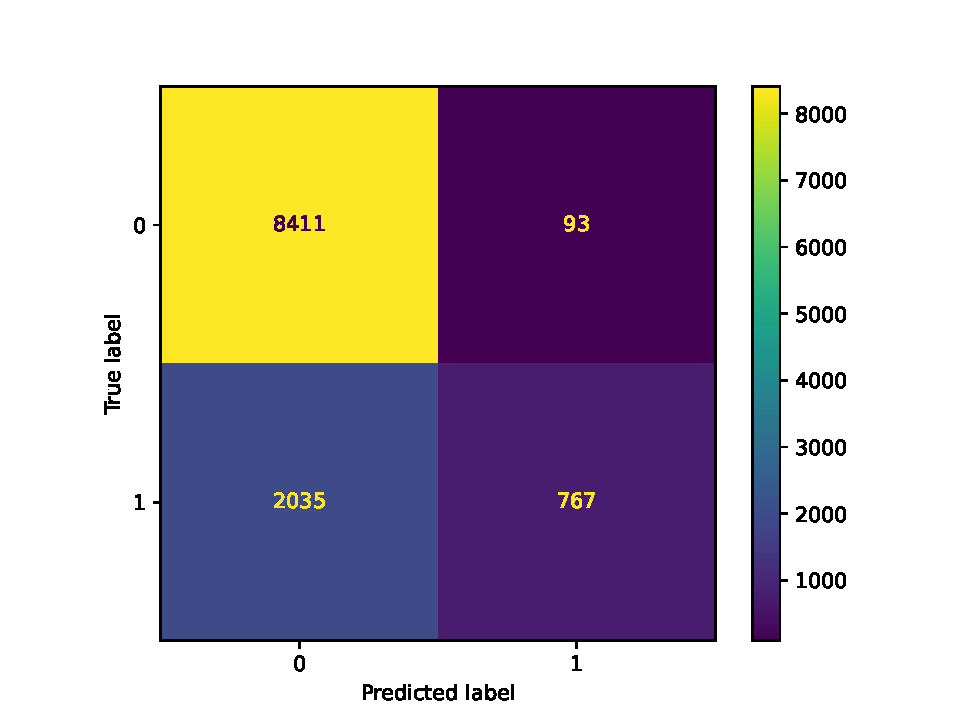
\includegraphics[width=.6\textwidth]{matrix_bag_of_trees.pdf} \\
        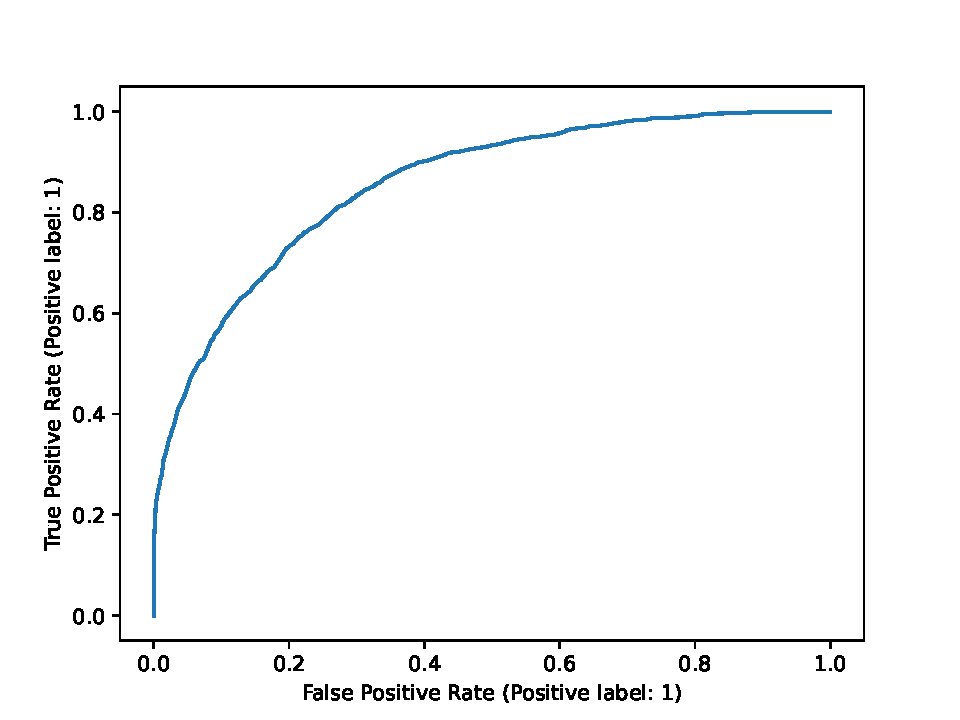
\includegraphics[width=.6\textwidth]{roc_curve_bag_of_trees.pdf}
    \end{center}
    \caption{Matriz de confusão e curva ROC para um \emph{bag of trees}. AUC = 0.856.}
    \label{bag of trees metric}
\end{figure}
Vemos que, apesar do \emph{recall} ter caído, todas as outras métricas subiram.

\subsubsection{\emph{Random Forest}}

O \emph{random forest} é um \emph{bag}, porém com uma tentativa de descorrelacionar as árvores.
Todas as considerações feitas para o \emph{bag of trees} se aplicam aqui.

Na Figura \ref{random forest metric} podemos ver a matriz de confusão e a curva ROC para este modelo.
As principais métricas do modelo foram:
\begin{itemize}
    \item \emph{Recall}: \( 46.9 \% \).
    \item Precisão: \( 72.27 \% \).
    \item Especificidade: \( 94.06 \% \).
    \item AUC: \( 0.855 \) (0.859 no treino).
\end{itemize}
\begin{figure}[htb]
    \begin{center}
        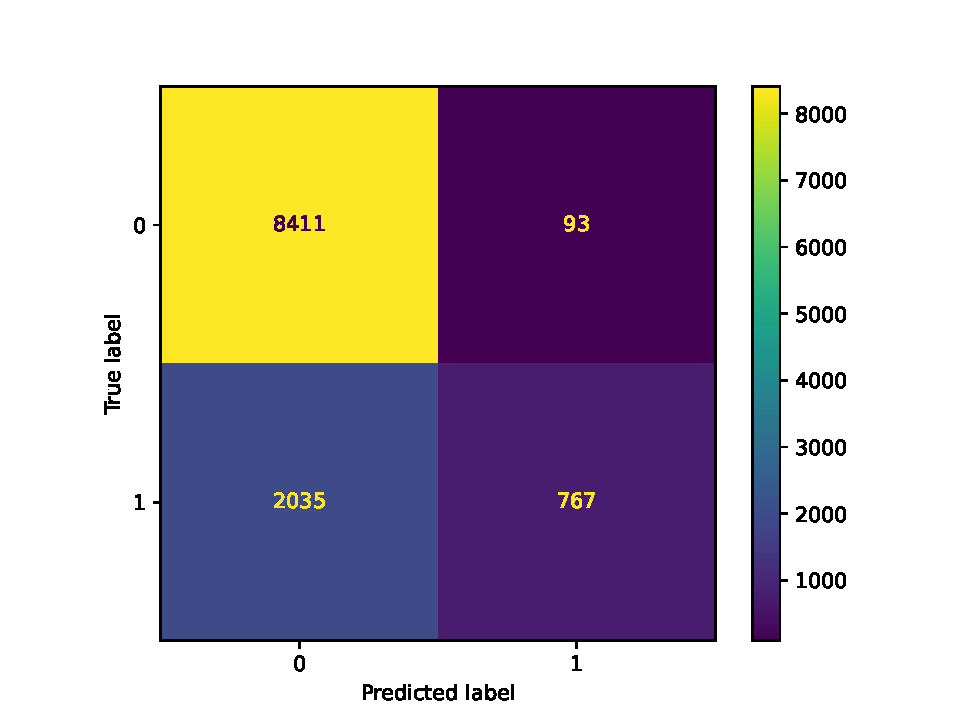
\includegraphics[width=.6\textwidth]{matrix_bag_of_trees.pdf} \\
        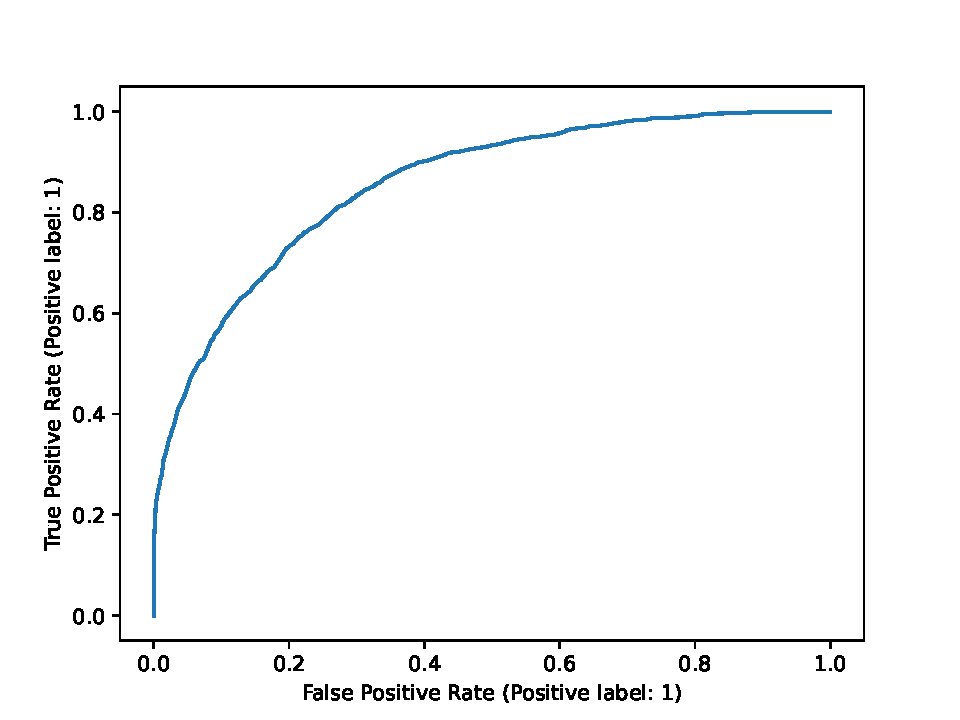
\includegraphics[width=.6\textwidth]{roc_curve_bag_of_trees.pdf}
    \end{center}
    \caption{Matriz de confusão e curva ROC para um \emph{bag of trees}. AUC = 0.856.}
    \label{random forest metric}
\end{figure}
Podemos ver que, apesar de uma queda na precisão e na especificidade com relação ao modelo de \emph{bagging}, houve um aumento do \emph{recall}, de modo que podemos concluir que o modelo ficou mais balanceado.

Para o \emph{random forest}, novamente temos uma forma prática de calcular as importâncias de cada \emph{feature}, já disponível como um método no \emph{Sci-Kit Learn}.
Ela é exatamente a mesma do classificador com apenas uma árvore.
As \emph{features} mais importamentes de acordo com essa métrica estão representadas na Figura \ref{random forest feature}.
\begin{figure}[htb]
    \begin{center}
        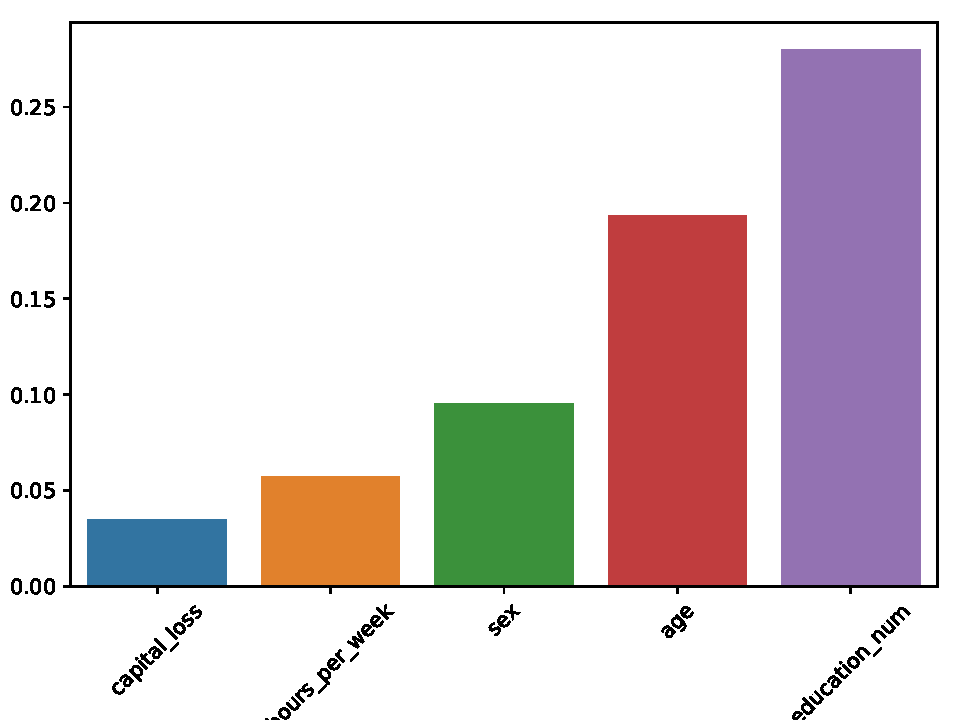
\includegraphics[width=.7\textwidth]{random_forest_feature_importances.pdf}
    \end{center}
    \caption{Features com maiores importâncias, de acordo com uma \emph{random forest}.}
    \label{random forest feature}
\end{figure}
Vemos que as conclusões são exatamente as mesmas obtidas quando consideramos apenas uma árvore.

\subsection{SVM}

As \emph{Support Vector Machines} são a classe de modelos mais complexa que consideramos.
Utilizamos um SVC (\emph{Support Vector classifier}) em conjunção com um \emph{scaler}.
Fizemos um \emph{grid search} para encontrar o melhor \emph{kernel} e parâmetro de regularização.
O resultado obtido foi um \emph{kernel} linear, com parâmetro de regularização \( C = 1 \) (veja a seção sobre regressão logística).
Como o \( SVM \) não gera probabilidades, a validação cruzada não foi realizada com a métrica AUC, e sim com a \emph{balanced accuracy score}, que, como dito na seção anterior, é a média entre o \emph{recall} e a especificidade.
As principais métricas do modelo foram:
\begin{itemize}
    \item \emph{Recall}: \( 85.55 \% \).
    \item Precisão: \( 57.70 \% \).
    \item Especificidade: \( 77.59 \% \).
    \item \emph{balanced accuracy score}: \( 0.816 \) (0.813 no treino).
\end{itemize}
Podemos ver que o modelo se saiu melhor no teste do que no treino.
Também vemos que ele apresenta um conjunto de métricas muito bom, comparado aos outros classificadores, por ser o único que conseguiu tanto \emph{recall} quanto especificidade elevados.
Na Figura \ref{svm metric} podemos ver a matriz de confusão para este modelo.
\begin{figure}[htb]
    \begin{center}
        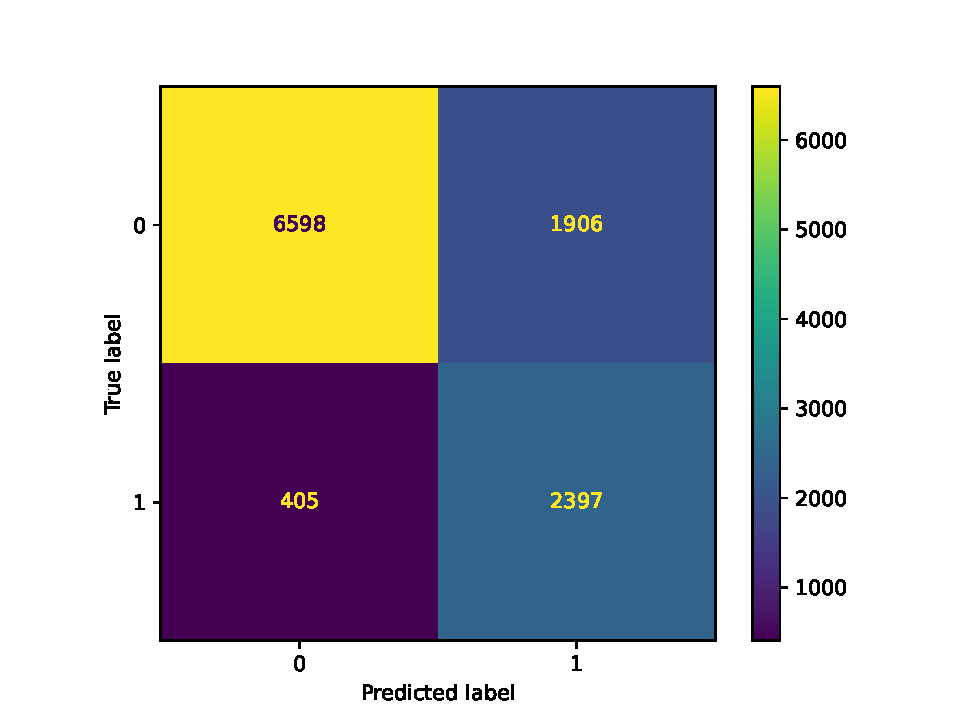
\includegraphics[width=.6\textwidth]{matrix_svm.pdf} \\
    \end{center}
    \caption{Matriz de confusão para o SVM.}
    \label{svm metric}
\end{figure}

\section{Conclusão}

Neste trabalho, nos propusemos a utilizar modelos de classificação para estudar o conjunto de dados \cite{uci}, com objetivo de prever/explicar a variável resposta, relativa à renda dos indivíduos.

Nesse sentido, na primeira parte realizamos uma análise exploratória, idenficando variáveis de interesse e possíveis problemas que deveríamos contornar.
Em primeiro lugar, nos deparamos com dados faltantes.
A solução utilizada para esse problema foi a de simplesmente desconsiderar os indivíduos que possuíssem alguma \emph{feature} latente.
Em segundo lugar, percebemos que o desbalanceamento do \emph{dataset} poderia criar um viés indesejado em favor da classe negativa.
Para contrabalancear essa tendência, utilizamos um mecanismo de pesos para cada classe, que demonstrou ser efetivo em quase todos os modelos analisados.

Ao treinarmos os classificadores, vimos que a estratégia de validação cruzada utilizada foi efetiva, pois as perdas nos conjuntos de treino e teste ficaram muito próximas.
Isto é, não houve overfitting significativo.
Também vimos que as \emph{features} que mais foram classificadas como relevantes foram: \verb|capital_gain|, o grau de educação, a idade e as relações conjugais de cada indivíduo.
A \emph{feature} \verb|capital_gain| é a única cujo significado não é inteiramente conhecido, por não ser informado na página do \emph{dataset}.
Por ser diferente de \verb|target|, podemos inferir que se trata de ganhos monetários além de salários.


\printbibliography

\end{document}

